\chapter[Resultados]{Resultados}

Baseando-se nos métodos e materiais descritos no capítulo \ref{chap:materials-and-methods}, iniciou-se a etapa de desenvolvimento e organização dos dados a partir da \textit{pipeline} de \textit{crappier} para a imagens, para então testar a hipótese do projeto. O presente capítulo mostra, de maneira detalhada, o que foi feito para realizar o levantamento e criação dos dados de imagens necessárias para serem consumidas pelos pré-processadores de imagem que visam melhorar a qualidade do OCR extraído dos textos, bem como a comparação dos mesmos por meio das métricas propostas.

\section{Infraestrutura}

Para o desenvolvimento do projeto foi utilizado um Sistema Operacional  Pop!\_OS 20.04 LTS baseado em GNU/Linux, com 16GB de memória RAM, disco com capacidade de 1.2 Terabytes de armazenamento, processador AMD® Ryzen 5 3600 com 6 (seis) \textit{cores} e 12 (doze) \textit{threads} e uma placa de vídeo dedicada NVIDIA GeForce RTX 2060 com 6GB de capacidade. Para os processamentos em placa gráfica foram utilizados o CUDA na versão 11.1 e o CuDNN na versão 7.


\section{Tratamento e formação do \textit{dataset}}

\subsection{Separação de documentos}
O conjunto de PDFs fornecidos como dados estavam todos juntos em um único diretório no disco, sem a correta divisão de qual era o dado contido no PDF. O CSV fornecido pelo GPAN e os itens descritos na tabela \ref{tab:csv-details} fazem referência a todas as páginas desses PDFs e possui também o seu conteúdo, sendo eles extraídos por meio de OCR ou não, como mostra a figura \ref{fig:gpan-pipeline}. Porém como o foco do trabalho é realizar estudos sobre a qualidade do OCR, decidiu-se por separar o dado entre os que foram extraídos utilizando OCR dos que não foram.

Para isso, gerou-se um novo CSV apenas com os registros de páginas cujo necessitou-se do OCR em sua extração e criou-se também um diretório para armazenar apenas os PDFs que possuíam páginas não-selecionáveis. Dos 89.578 arquivos, existem cerca de 354.501 páginas somadas, sendo essas:

\begin{table}[H]
  \centering
  \caption{Divisão de páginas dos PDFs.}
  \begin{tabular}{|m{10em}|c|}
    \hline
      \textbf{Tipo}  &
      \textbf{Quantidade} \\
    \hline
      Necessita de OCR  &
      80.624 \\
    \hline
      Não necessita de OCR  &
      273.877 \\
    \hline
      \textbf{TOTAL}  &
      \textbf{354.501} \\
    \hline
  \end{tabular}
  \legend{Fonte: autoral}
  \label{tab:csv-diff}
\end{table}

\subsection{Extração de imagem do PDF}
Com os dados separados em um diretório específico, iniciou-se a etapa de extração de imagem a partir dos documentos em formato PDF dos processos. Utilizou-se também informações do CSV (tabela \ref{tab:csv-details}) para selecionar a página específica do documento a qual o OCR foi utilizado, diminuindo assim o tempo de processamento por documento.

A extração de imagem a partir do PDF é feita utilizando um algoritmo de software livre desenvolvido em Python, chamado de \textit{pdf2image}. Ele recebe como entrada um PDF e é possível definir qual ou quais páginas do PDF deseja-se extrair, permitindo assim a geração do \textit{dataset} de imagens de processos.

\subsection{Aplicação de filtros}
Para a criação de um modelo generativo que consiga diminuir os ruídos de imagens, é preciso utilizar como dado de entrada imagens que possuam tais características - ruídos. Das 354 mil páginas dos PDFs disponíveis, fazer a separação de todas elas para a identificação de imagens ruins deria um trabalho bem complexo e que diminuiria o tempo disponível para o desenvolvimento do presente trabalho. Com isso, adotou-se a heurística de que todas as fotos que tiveram texto extraído via OCR (tabela \ref{tab:csv-diff}) seriam "pioradas" \  aplicando um conjunto de filtro de imagens de diferentes tipos.

Um filtro de imagem é um algoritmo ou rotina de software que consegue alterar de forma fixa ou aleatória os valores dos pixels contidos em uma imagem. Com isso, é possível criar uma lógica que tente simular imagens escaneadas de maneira automatizada, aplicando sombreamento, borrões, manchas, distorções, etc.


\begin{figure}[H]
  \centering
  \caption{Diferença entre uma foto original e uma com filtro}
  \begin{subfigure}{.5\textwidth}
    \centering
    \caption{Foto sem filtro}
    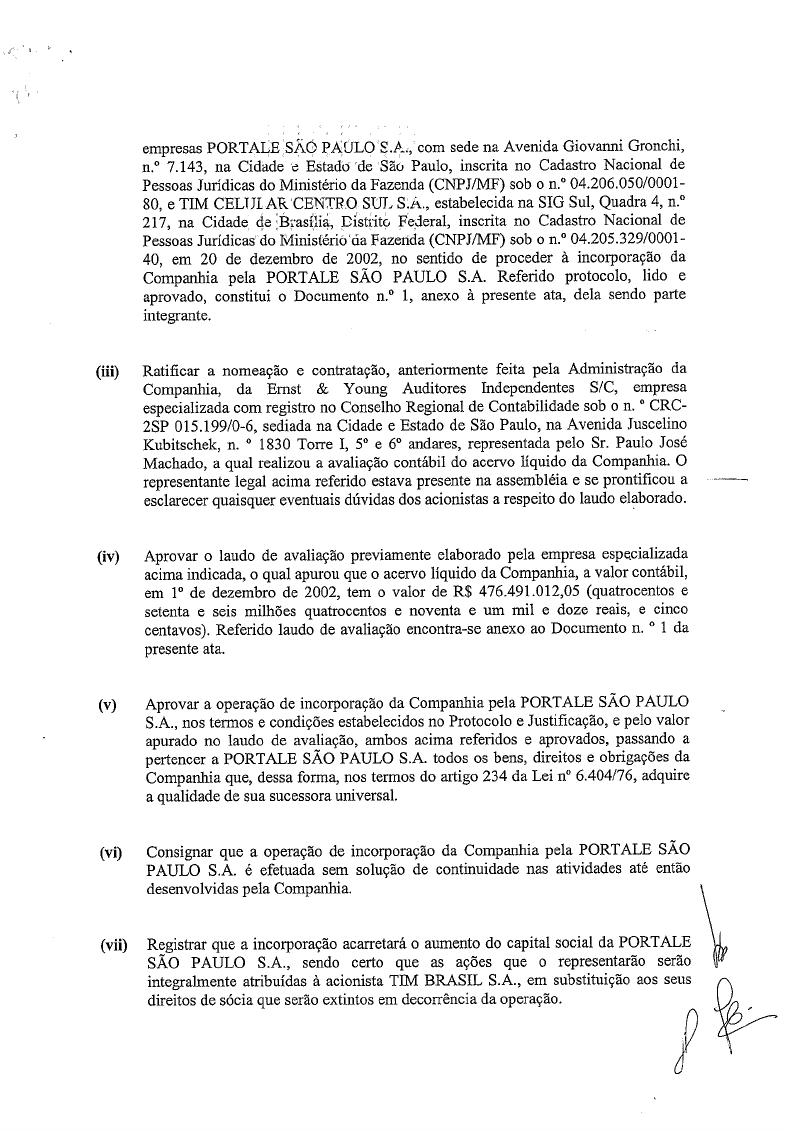
\includegraphics[width=0.8\linewidth]{figuras/good-text-image.jpg}
    \label{fig:image-without-filter}
  \end{subfigure}%
  \begin{subfigure}{.5\textwidth}
    \centering
    \caption{Foto com filtro aplicado}
    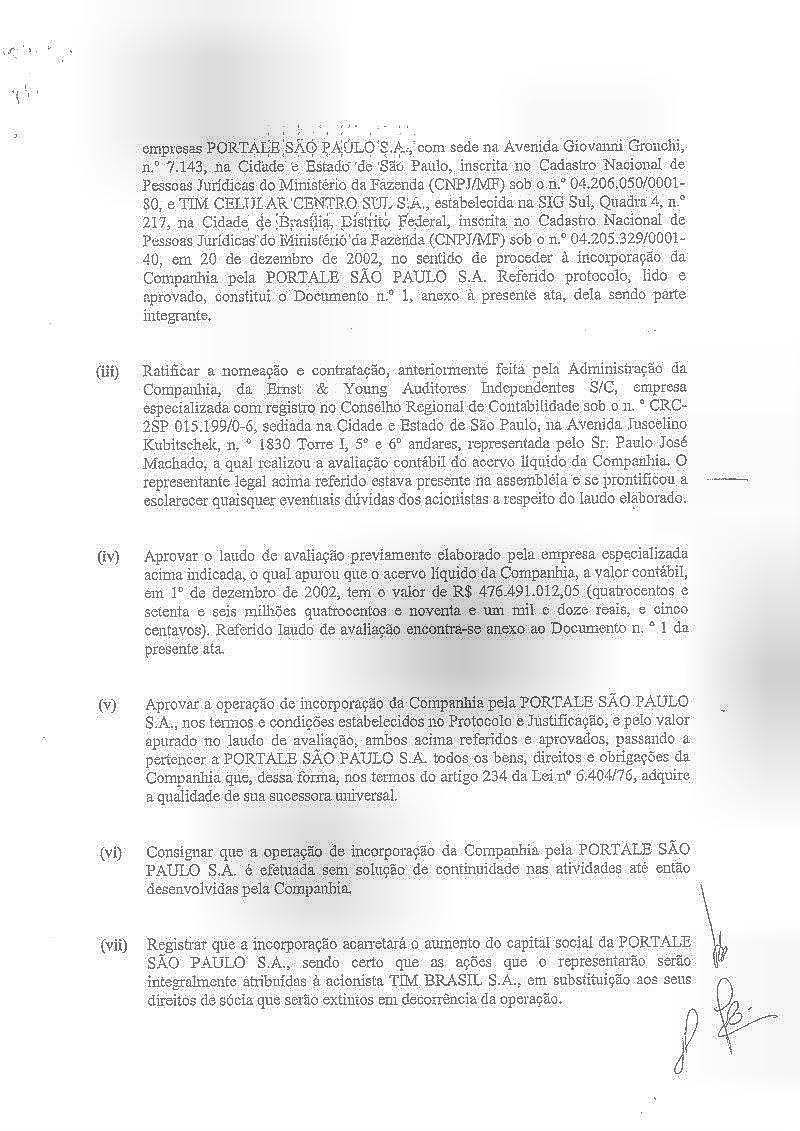
\includegraphics[width=0.8\linewidth]{figuras/image-with-overlay.jpg}
    \label{fig:image-with-filter}
  \end{subfigure}
  \legend{Fonte: autoral}
  \label{fig:side-process-images}
\end{figure}

Existem diversas bibliotecas já implementadas em Python que possibilitam a aplicação de filtros em imagens. As utilizadas foram: \textit{ImageFilter} da biblioteca \textit{Python Imaging Library} e \textit{imgaug}, biblioteca de \textit{data augmentation}\footnote{
  Processo de transformação do dado que permite que seu volume ou amostra cresça, fornecendo assim mais insumos ou entradas de dados disponíveis em um processo de treinamento de algoritmo.
}. Alguns filtros foram de origem autoral.

Abaixo, listam-se todos os filtros utilizados e estudados para o presente processamento de imagem.

\begin{table}[H]
  \centering
  \caption{Descrição dos filtros utilizadosverbo tesselar.}
  \begin{tabular}{|m{.25\linewidth}|m{.1\linewidth}|m{.55\linewidth}|}
    \hline
      \textbf{Nome}  &
      \textbf{Fonte}  &
      \textbf{Descrição} \\
    \hline
      EDGE\_ENHANCE  &
      PIL  &
      Aumenta o contraste dos píxels ao redor de bordas para que essas bordas se destaquem mais do que os demais elementos da foto  \\
    \hline
      CONTOUR  &
      PIL  &
      Similar ao EDGE\_ENHANCE mas com maior intensidade \\
    \hline
      RandomOverlay  &
      autoral  &
      Cria formas gerométricas randômicas e transparentes e as coloca acima da imagem original, dando a impressão de manchas. A posição das formas também é randômica. \\
    \hline
      PerspectiveTransform  &
      \textit{imgaug}  &
      Aplica randomicamente transformações de 4 pontos de perspectiva, dando uma ideia de "lupa" para algus pontos da imagem \\
    \hline
      SaltAndPepper  &
      \textit{imgaug}  &
      Substitui píxels randômicos da imagem por píxel de sal (cor branca) e pimenta (cor preta) \\
    \hline
      GammaContrast  &
      \textit{imgaug}  &
      Ajusta o contraste da imagem escalando os píxels da imagem em um valor calculado por \(x = 255(\frac{v}{255})^{\gamma}\), onde $\gamma$ é um parâmetro da função entre $0$ a $1$ e $v$ é o antigo valor do píxel \\
    \hline
      JpegCompression  &
      \textit{imgaug}  &
      Degrada a imagem aplicando uma compressão de JPEG, diminuindo sua qualidade \\
    \hline
      Dropout  &
      \textit{imgaug}  &
      Randomicamente coloca uma fração de pixels da imagem para o valor 0 \\
    \hline
      Affine  &
      \textit{imgaug}  &
      Aplica transformações na imagem mas mantém relações de colinearidade e distância. Geralmente composta por rotações, translações e dilatações das formas presentes na imagem. \\
    \hline
  \end{tabular}
  \legend{Fonte: autoral}
  \label{tab:sdas}
\end{table}

As tecnologias de OCR disponíveis, como o Tesseract, em geral são muito sensíveis e aplicar todos esses filtros em uma única imagem impede que o OCR identifique caracteres nas mesmas. Com isso, é preciso escolher randomicamente entre os filtro listados, podendo aplicar um ou mais deles, mas nunca podendo aplicar todos de uma só vez.

O processo seguido para a criação de imagens ruins foi de que, para cada uma imagem boa, gera-se uma imagem ruim. Isso se dá pela alta quantidade de imagens disponíveis para treinamento, visto que se for necessário o consumo de mais imagens para treinamento na etapa de geração do modelo, é possível utilizar de \textit{data augmentation} para ampliar a base de dados.

\begin{figure}[H]
  \centering
  \caption{Geração de imagens atual vs geração com \textit{data augmentation}}
  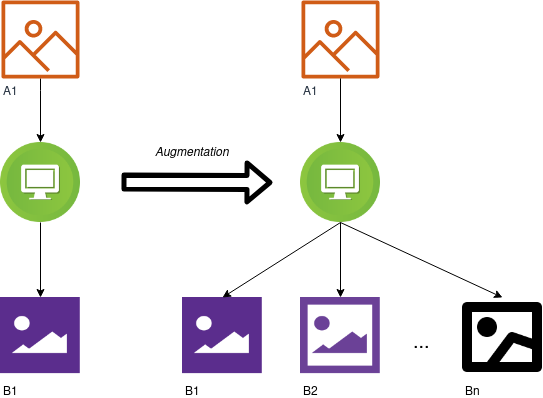
\includegraphics[scale=.6]{figuras/data-augmentation.png}
  \legend{Fonte: autoral}
  \label{fig:data-augmentation}
\end{figure}

\subsection{Extração de texto via OCR}

Para a extração de caracteres utilizando o OCR, fez-se o uso da tecnologia Tesseract, que atualmente consegue identificar e reconhecer mais de 100 idiomas por meio da configuração \textit{unicode}\footnote{
  Padrão que permite que os sistemas informatizados representem e manipulem textos de quaisquer idiomas de escrita que existem na atualidade. Fonte: Wikipedia.
}. Para tal, configura-se o Tesseract com a extensão para a lingua portuguesa, já disponível pela comunidade para uso.

Todo o texto extraído é armazenado em um CSV de saída que identifica qual o processo, documento e página que a extração foi feita. Isso depois servirá como base para a verificação e métrica para a comparação entre o texto extraído de uma página limpa para uma página com ruídos.

O texto extraído das imagens ruins foram comparados previamente para verificar se o OCR estava realmente pior do que o texto original, a partir da métrica ROUGE-1. A seguir, mostra-se um exemplo de imagens e suaas respectivas extrações de texto utilizando OCR, sendo a primeira da imagem original e a segunda da imagem \textit{crappy}, respectivamente.

\begin{figure}[H]
  \centering
  \caption{Imagem de boa qualidade}
  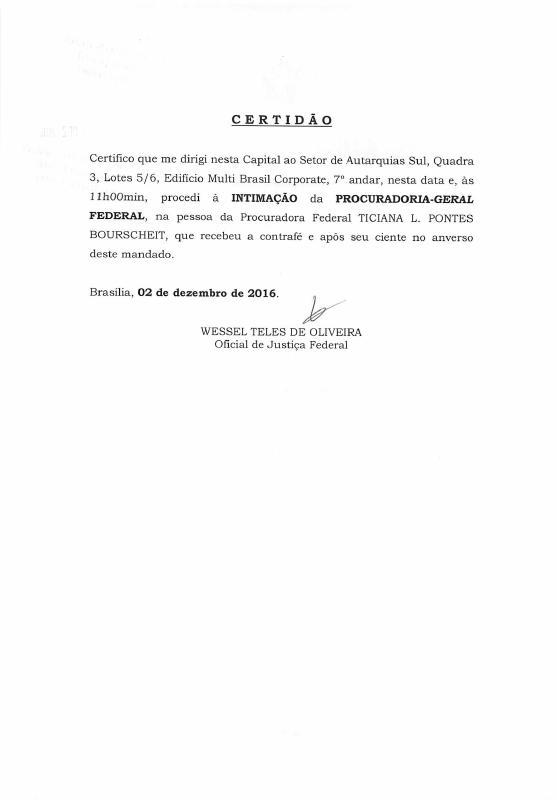
\includegraphics[scale=.6]{figuras/good-image-extracted.jpg}
  \legend{Fonte: STF.}
  \label{fig:good-image-extracted}
\end{figure}

\begin{alltt}
          CERTIDÃO

          Certifico que me dirigi nesta Capital ao Setor de
          Autarquias Sul, Quadra 3, Lotes 5/6, Edificio Multi
          Brasil Corporate, 7º andar, nesta data e, às
          11h00min, procedi à INTIMAÇÃO da PROCURADORIA-GERAL
          FEDERAL, na pessos da Procuradora Federal TICIANA L. PONTES
          BOURSCHEIT, que recebeu a contrafé e após seu
          ciente no anverso deste mandado.

          Brasília, 02 de dezembro de 2016,

          WESSEL TELES DE OLIVEIRA
          Oficial de Justiça Federal
\end{alltt}

\begin{figure}[H]
  \centering
  \caption{Imagem gerada pelo \textit{crappier} \textit{pipeline}}
  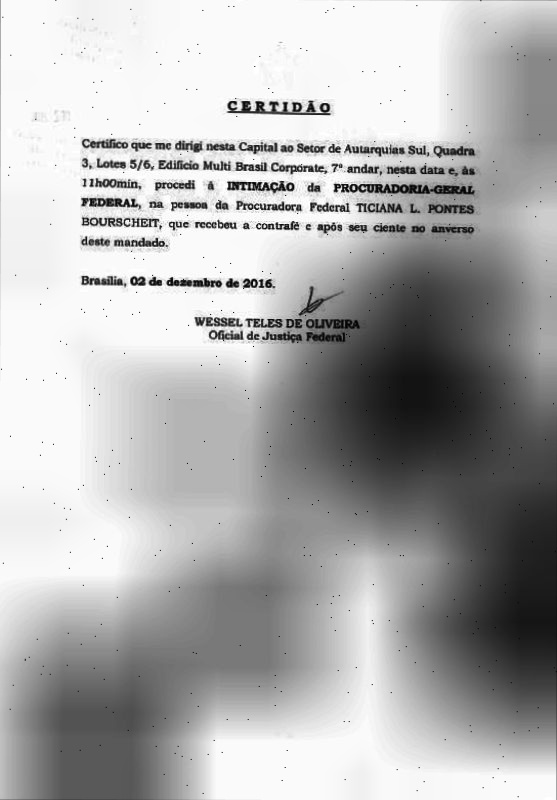
\includegraphics[scale=.6]{figuras/bad-image-extracted.jpg}
  \legend{Fonte: autoral.}
  \label{fig:bad-image-extracted}
\end{figure}

\begin{alltt}
          CERTIDÃO

          Certífico que me dirigi nesta Capital ao Setor de
          Autarquias Sul, Quadra. 4 , Lotes 5/6, Edifício Muki
          Brasil Corpórate, 7º andar, nesta
          11h00Min, procedi à INTIMAÇÃO da
          FEDERAL, na pesson da Procuradora Federal TICIANA
          BOURSCHEIT, que recebeu a contrafé e apõs sem
          deste mandado.

          Brasília, 02 de desembro de 2016.
\end{alltt}

Foi possível então verificar, assim como no exemplo acima, que a qualidade de extração do OCR piorou em comparação com o texto original. Neste exemplo, ao ser aplicada a métrica ROUGE-1, obteve-se como \textit{score} o valor de $0.65$, mostrando que existem diferenças significativas dentro do texto.

Permite-se então validar que o \textit{dataset} gerado poderá servir de insumo para as etapas futuras do desenvolvimento do projeto.

\section{Pré-processadores de Imagem}

Com todo o \textit{dataset} devidamente construído, é possível prosseguir com a construção dos pré-processadores de imagens. Para validar os estudos propostos, criou-se 3 (três) tipos diferentes de processadores:

\begin{itemize}
  \item Processador de Imagem simples;
  \item Processador GAN;
  \item Processador \textit{Decrappification};
\end{itemize}

\begin{figure}[H]
  \centering
  \caption{Processo de correção de imagem, extração de texto e criação de métricas}
  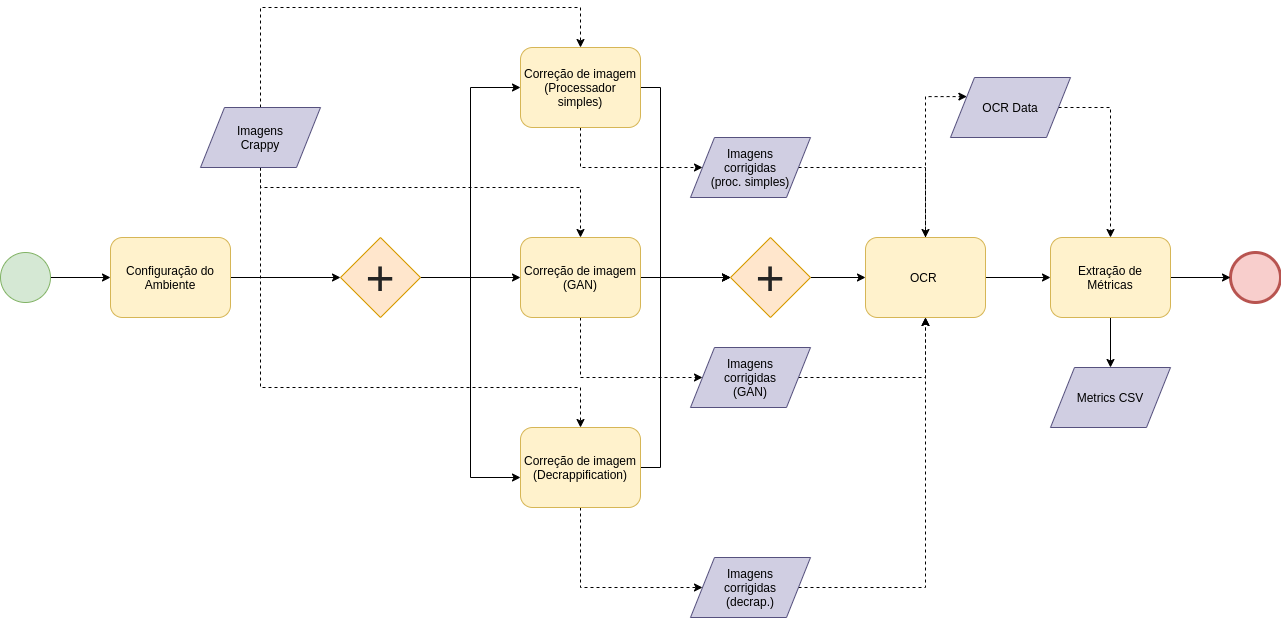
\includegraphics[scale=.5, angle=270]{figuras/text-extraction-and-comparison-flow.png}
  \legend{Fonte: autoral.}
  \label{fig:text-extraction-and-comparison-flow}
\end{figure}

O processo de construção dos mesmos, bem como exemplos de seus resultados serão apresentados a seguir.

\subsection{Pocessador de Imagem simples}
\subsection{Pocessador GAN}
\subsection{Pocessador \textit{Decrappification}}
\subsection{Extração de Métricas}
\subsection{Comparação de resultados}